\documentclass[12pt]{article}
\usepackage[utf8]{inputenc}
\usepackage[left=2.5cm,right=2.5cm,top=2.5cm,bottom=2.5cm]{geometry}
\usepackage{cite}

\usepackage{amsmath,amssymb,amsfonts,amsthm}
\newtheorem{theorem}{Theorem}
\newtheorem{cor}[theorem]{Corollary}
\newtheorem{lemma}[theorem]{Lemma}
\newtheorem{conjecture}[theorem]{Conjecture}
\newtheorem{prop}[theorem]{Proposition}
\newtheorem{claim}{Claim}
\theoremstyle{definition}
\newtheorem{definition}{Definition}
\newtheorem{remark}{Remark}
\newtheorem{assumption}{Assumption}
\newtheorem{corollary}{Corollary}
\newtheorem{example}{Example}
\DeclareMathOperator*{\argmax}{arg\,max}
\DeclareMathOperator*{\argmin}{arg\,min}

\usepackage{gensymb}
\usepackage{multirow}
\usepackage{multicol}
\usepackage{caption}
\usepackage{comment, bm, enumerate}
\usepackage[ruled,vlined]{algorithm2e}
\usepackage{subfigure}

\usepackage{graphicx}
\usepackage{wrapfig}
% Example for wrapping text around a figure 
% \begin{wrapfigure}{R}{0.3\textwidth}
% \centering
% \includegraphics[width=0.25\textwidth]{path_to_your_figure}
% \caption{\label{label_of_your_figure}This is a figure caption.}
% \end{wrapfigure}

\usepackage{subfig}
% Example for including multiple images into one figure
% \begin{figure}
%      \centering
%      \begin{subfigure}[b]{0.3\textwidth}
%          \centering
%          \includegraphics[width=\textwidth]{path_to_your_graph1}
%          \caption{caption_of_your_graph1}
%          \label{label_of_your_graph1}
%      \end{subfigure}
%      \hfill
%      \begin{subfigure}[b]{0.3\textwidth}
%          \centering
%          \includegraphics[width=\textwidth]{path_to_your_graph2}
%          \caption{caption_of_your_graph2}
%          \label{label_of_your_graph2}
%      \end{subfigure}
%      \hfill
%      \begin{subfigure}[b]{0.3\textwidth}
%          \centering
%          \includegraphics[width=\textwidth]{path_to_your_graph3}
%          \caption{caption_of_your_graph3}
%          \label{label_of_your_graph3}
%      \end{subfigure}
%         \caption{Three graphs example}
%         \label{fig:three graphs}
% \end{figure}

\usepackage[dvipsnames]{xcolor}
\usepackage[T1]{fontenc}
\usepackage{hyperref}
\hypersetup{
    colorlinks=true,
    linkcolor=blue,
    filecolor=magenta,      
    urlcolor=cyan,
    pdftitle={Overleaf Example},
    pdfpagemode=FullScreen,
}

\usepackage{booktabs, caption, makecell}
\usepackage{threeparttable}

%Copy code
\usepackage{listings}
\lstset{basicstyle=\footnotesize\ttfamily,breaklines=true}
\lstset{framextopmargin=50pt,frame=bottomline}

% Default BibTeX in apalike style, activate the following line:
\bibliographystyle{apalike}
% If you use natbib package, activate the following three lines:
\usepackage[round]{natbib}
\renewcommand{\bibname}{References}
\renewcommand{\bibsection}{\subsubsection*{\bibname}}

\title{Kaggle InClass Competition Report - Airbnb Prediction Track}
\author{Rajas Pandey\\
Kaggle username - Rajas Pandey
}
\date{\today \\
%\href{}{Link} 
}

\usepackage{hyperref}
\usepackage{graphicx}

\begin{document}

\maketitle

I have done the Kaggle Prediction challenge on the Airbnb dataset.

My predictions achieved a Misclassification error of 0.28005 on the Leaderboard evaluation dataset. 
\section{Exploratory Analysis}
The first step after looking at the data file was to understand the columns and what they mean. I have attached my code with detailed comments for this analysis in the appendix. To start with, I tried to understand each feature and it's datatype by browsing through it on Excel. This gives me a sense of what sort of values are there in each column, what each column means and I can start to form hypothesis about the importance of various features for the classification problem of interest. \\

Around 63\% of the training data has a positive Decision value.

\subsection{NA analysis}
I observed some columns had missing values, so my first thought was to understand what's going on there. The main question I wanted to answer was whether the missing values were missing at random (possibly due to a data pipeline issue) or were they missing structurally. To observe that, I plotted the a correlation heatmap of just the null values \ref{fig:na_heatmap}.\\

From here, I observed that most of the host identification attributes are missing when \texttt{Host\_is\_superhost} is missing. This means that all the 3 identifying attributes are linked and must be imputed together. As they are all 't'/'f' values, I impute them with False.\\


\begin{figure}
\centering
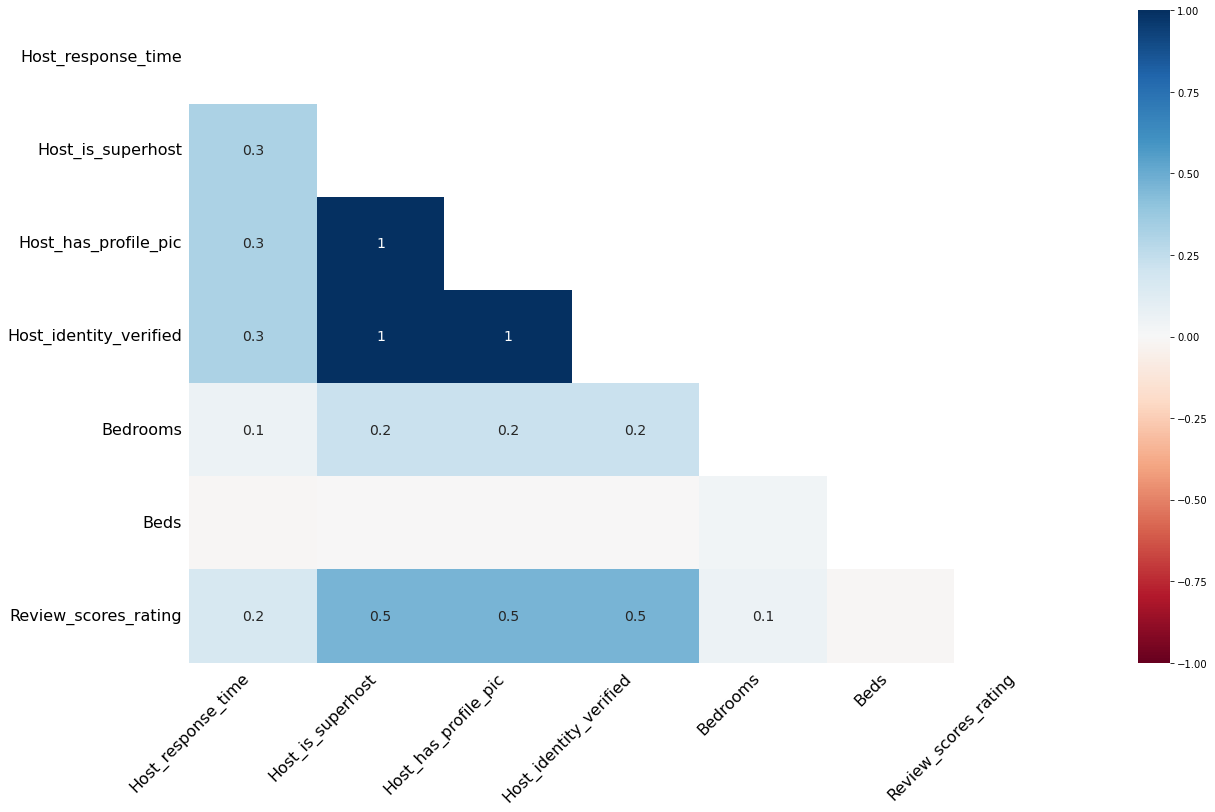
\includegraphics[width=0.7\textwidth]{kaggle_figs/1. na_heatmap.jpg}
\caption{\label{fig:na_heatmap}Which NA values occur together? Example, all missing values of \texttt{Host\_has\_profile\_pic} occur when \texttt{Host\_is\_superhost} is also missing}
\end{figure}

\begin{wrapfigure}{R}{0.5\textwidth}
\centering
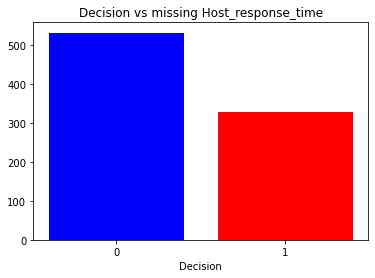
\includegraphics[width=0.5\textwidth]{kaggle_figs/2.missing_vs_host_resp.png}
\caption{\label{fig:missing} What Decision values do rows with missing Host\_response\_time have? }
\end{wrapfigure}


The feature with most number of attributes missing is Host\_response\_time \ref{fig:missing}. So I check how the Decision values are distributed in the missing data. The missing values have a significantly higher distribution of Decision 0 compared to the dataset. Thus, these values are critically important and should not be dropped. I hypothesize that the missing values in this attribute are because of new host (at least a third of these hosts don't have their identities verified either, from \ref{fig:na_heatmap}). So the correct imputation will be to assign 0 to the missing values.\\

All this analysis used Pandas\cite{pandas} and Matplotlib\cite{matplotlib} libraries. Similar analysis is also done for other features, which is present in the appendix. 

\subsection{Data Prerpocessing}
The next logical step after NA analysis is to deal with the NA values. There are also some categorical features, which aren't readily read by ML models. 

\subsubsection{NA value imputation}
\texttt{Host\_response\_time} - Fill NA with blank\\
The rationale is that when encoding the categorical variable, it will automatically assign a category to the blank value as well.\\

\texttt{Host\_is\_superhost} - Fill NA with false\\
\texttt{Host\_ has\_profile\_pic} - Fill NA with false\\
\texttt{Host\_has\_identity\_verified} - Fill NA with false\\
The rationale is that most of these values may be missing due to new host. So in that context, the NAs should ideally represent false.\\

\texttt{Bedrooms} - Fill NA with 0\\
\texttt{Beds} - Fill NA with 0\\
A similar rationale to identity attributes is hypothesised here. New houses or houses with 0 Beds or Bedrooms will have NA in these places. So imputed with 0 values there.

\subsubsection{Encoding}
Two types of encodings are used - LabelEncoding and One-Hot Encoding.

Label encoding is used when there is an ordinal relation between the categorical attributes. For example, in the \texttt{Host\_response\_time} feature, there is an inherent ordering in the time the host takes to respond. So that and all the other binary (including true false) variables are Label encoded. Label encoder assigns unique numeric values to each category and preserves ordinal relationship.\\

One hot encoding is used when there is no ordinal relationship between the categories. One hot encoding creates a new binary column for each category. This encoding has been used for categorical attributes like Neighbourhood, Month and Room\_type where there is no ranking between the categories. \\

A challenge while using one-hot encoding is that there might be multi-collinearity between the new created features. This is avoided by dropping the first category. This implies that 0 values for all the other created attributes implies that it must be the first category. 

\subsubsection{Feature engineering}
\texttt{Bathroom\_text} feature had a string of values. Some of them had numeric values and string descriptors. An example of such values is "1.5 shared bathrooms" or "Private half-bath". I created 2 new columns - \texttt{Num\_baths} and \texttt{Shared\_bath} and split the information from the Bathroom Text column. The numerical part, including text numbers like "half" was stored as a float in the \texttt{Num\_baths} column. \texttt{Shared\_bath} is a binary column indicating whether it is a shared bath or not. This was done to better incorporate the information in a machine ready format\\

The Price column was also processed to use the float value of the price. 





\section{Methods}
\subsection{Models}
I used 3 basic classifiers and a Stacked classifier for my final predictions. 
\subsubsection{Support Vector Machines}
I used SVM because it is usually a good model for high-dimensional spaces. Though the computation costs are higher comparatively, the small size of the training data ensured that it was not too long. In the case of binary classification, there is the separating hyper plane intuition of SVM which is convenient to visualise and understand.\\

Further, I used the SVM with RBF kernel. RBF kernels are easy to tune and have a small number of Hyperparameters. Only Hyperparameters in RBF kernels are C and gamma, which I tuned using cross validation. \\

In addition, SVMs were recently covered in class and homeworks so I was confident of debugging with them.\\

\subsubsection{Random Forest}
Random Forests are based on decision trees and pick certain features randomly while creating a tree. Finally, it takes the vote of all the tree classifiers to determine the final class. As they are based on decision trees, Random Forests are really fast to train. They have several parameters like \texttt{max\_features}, \texttt{min\_samples\_split} and \texttt{n\_estimators} which can be tuned.\\

Usually, Random Forests tend to do well because of the randomisation at each level of the tree creation and the eventual voting. Ed Tam mentioned in his Discussion class that Random Forests are usually the second best algorithm for every classification task after the specific algorithm for that task.

\subsubsection{Logistic Regression}
Logistic Regression is again a useful algorithm for binary classification. It is also very easy to tune Logistic Regression hyper-parameters - there is just the regularisation penalty. I use l2 regularisation which has 1 hyper-parameter C and I tune it using cross validation.\\

Logistic regression also has a nice intuition for binary classification, in terms of the sigmoid value being closer to 0 or 1 (the value of the function being positive or negative).  
\subsubsection{Stacking}
Finally, I got the best results for Stacking classifier. Stacking runs the estimators (logistic, random forest and svm) independently and then trains another classifier (in my case, a logistic regression) on the output of the estimators to predict the correct outcome. \\

This is similar to voting in random forest type algorithms. My goal was to reduce the bias in the algorithms, and Stacking is a way to combine the good parts of different algorithms.Unlike voting, in stacking, the final estimator learns the importance of each estimators output on the overall prediction, improving the quality of the result. 


\subsection{Training}
\subsubsection{SVM}
I decided to use the RBF kernel for the reasons mentioned above. I was training on the Kaggle notebook using the CPU.\\

Before training SVM, it is very important for the data to be in the same scale. I used a StandardScaler which uses mean and variance to scale each observation. This is part of a pipeline, which executes every time SVM model is trained. \\

I ran a GridSerach over C and gamma parameters in the logspace (-4,4) based in Numpy \cite{numpy} with a step of 5. There were total 25 values of C and gamma which the algorithm iterated over. The algorithm I used was scikit-learn \cite{scikit-learn} SVC which is based on libsvm. \\

For each value, I used a 10-fold cross validation as a GridSearch parameter. I also leverage the inbuilt paralleization in gridsearch to use the max number of concurrent workers available. This significantly speeds up the training process for SVM which is usually long.\\

\subsubsection{Random Forest}
Here too I use gridsearch to estimate the hyperparameters using cross validation. The data is split up into 10 cross validation folds and the class weights are set to 'balanced\_weights'. This setting of class weights is useful when there is imbalance among classes as is the case in our dataset.\\

Gridsearch in turn uses the scoring rule accuracy as we want to maximise the accuracy of our predictions. \\

\subsubsection{Logistic Regression}
LogisticRegressionCV is already implemented in sklearn and I used it directly. I used the 'l2' penalty and 'liblinear' solver which is considered to be good\footnote{\url{https://scikit-learn.org/stable/modules/generated/sklearn.linear_model.LogisticRegressionCV.html}} for binary classification when there are cases of 1 vs all. \\

Here too, I run it over 10 cross validation folds. The only hyperparameter here is the C or regularization parameter. The best value for C is observed to be 10.\\

\subsubsection{Stacking}
While Stacking, I use the algorithms with their best parameters determined by cross validation. The final estimator in the scikit-learn Stacking implementation is Logistic Regression, which is used as is out of the box. Stacking classifier trains the fastest because there is no cross-validation used here. \\

The following table shows the training time comparisons of the various classifiers I have used. Logistic regression is the fastest to train, followed by Stacking which uses just the best cross validated parameters.

\begin{center}
\begin{tabular}{|l|l|}
\hline
                    & Average training time (s) \\ \hline
Stacking            & 19.57                     \\ \hline
SVM                 & 569.41                    \\ \hline
Random Forest       & 131.18                    \\ \hline
Logistic Regression & 4.29                      \\ \hline
\end{tabular}
\end{center}
\ref{fig:train-compare} shows that Random Forest overfits on the training data and has a very high training accuracy. 
\begin{figure}[!htbp]
    \centering
    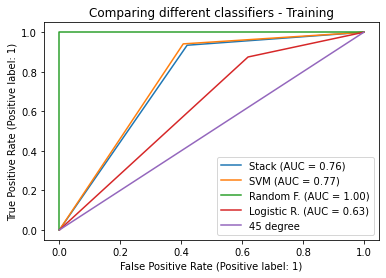
\includegraphics[width=0.6\textwidth]{kaggle_figs/train_comparing_classifiers.png}
    \caption{Comparing classifier training ROC curves}
    \label{fig:train-compare}
\end{figure}


\subsection{Hyper-parameter Selection}
\subsubsection{SVM}
The two hyper-parameters under consideration were C and gamma in the RBF kernel. \ref{fig:val_acc} shows the accuracy changing with C and Gamma. The best parameters were found to be C = 100 and gamma = 0.01.\\



\begin{figure}[h]
    \centering
    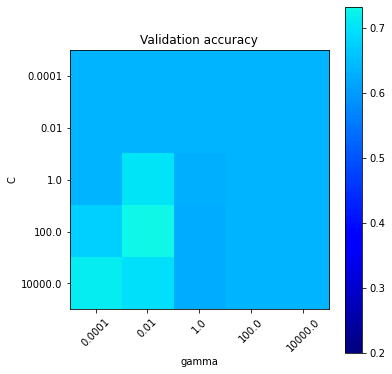
\includegraphics[width=0.5\textwidth]{kaggle_figs/validation_acc.png}
    \caption{Validation set accuracy with C and Gamma}
    \label{fig:val_acc}
\end{figure}
C is the penalty associated with the regularisation term and controls the error. Higher C usually implies more error. Gamma is a parameter of the RBF kernel and is used to control the curvature of the decision boundary. Lower gamma boundaries are more curved, while higher gamma boundaries are more spread\footnote{\url{https://medium.com/@myselfaman12345/c-and-gamma-in-svm-e6cee48626be}}. 

\subsubsection{Random Forest}
The parameters used are n\_estimators and max\_features. We iterate over values of n\_estimators from 100 to 500. This parameter represents the number of decision trees to be constructed during the training. \\

More trees often leads to more accuracy. However, the computation time also significantly increases with more trees. The best value was found to be 400 trees. \\

max\_features parameter represents how many features should be considered in each iteration of the tree. I have iterated over 2 values - None and 'sqrt'. None means no restrictions on the number, it can theoretically consider all the features that it finds best. 'sqrt' parameter consideres only the square root of the number of features available at any time. Further implementation is in the appendix.

\subsubsection{Logistic Regression}
Only the C hyperparameter which is tuned by LogisticRegressionCV function on its own. It represents penalty and is similar to the C in SVM. 

\subsubsection{Stacking}
No hyperparameters tuned here. Only the best parameters from all the previous algorithms are used to train this model.

\section{Results - Prediction}

The objective of the prediction task was to get the lowest Mean Absolute Error. In my case, that was achieved in the Stacking classifier using Logistic regression, SVM and Random Forest stacked together. \\

The following table shows the performance of these classifiers on the validation set - 
\begin{center}
    \input{kaggle_figs/error_table}
\end{center}

We can further compare the classifiers using their ROC curves and AUC. This is presented in \ref{fig:roc}.\\

There is a quirky observation that although Random Forest seems to perform better on the validation set, it fails to do as well on the actual unseen data on Kaggle. This may be because training and validation sets are from the same distribution, so there are higher chances of Random forest learning and sort of overfitting on the training data. \\

I further investigate the observations on which the algorithms perform well. In particular, I look at the confusion matrices \ref{fig:cm} and observe that Random Forest is predicting 0 labels much better than all the other algorithms. Perhaps this is why it was giving higher accuracy. \\

\begin{figure}
    \centering
    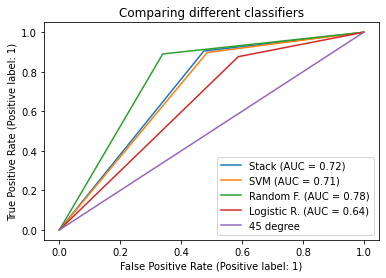
\includegraphics[width = 0.6\textwidth]{kaggle_figs/comparing_classifiers.png}
    \caption{Comparison of ROC of different classifiers on the Validation set}
    \label{fig:roc}
\end{figure}

\begin{figure}[!htbp]
     \centering
     \begin{minipage}{0.4\textwidth}
         \centering
         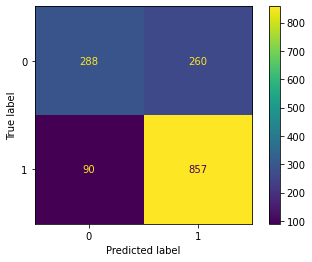
\includegraphics[width=\textwidth]{kaggle_figs/stack_cm.png}
         \subcaption{Stacked classifier}
         \label{fig:stack_cm}
     \end{minipage}
     \begin{minipage}{0.4\textwidth}
         \centering
         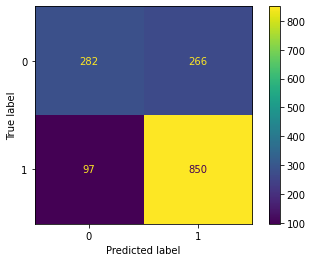
\includegraphics[width=\textwidth]{kaggle_figs/svm_cm.png}
         \subcaption{SVM classifier}
         \label{fig:svm_cm}
     \end{minipage}
     \vskip\baselineskip
     \begin{minipage}{0.4\textwidth}
         \centering
         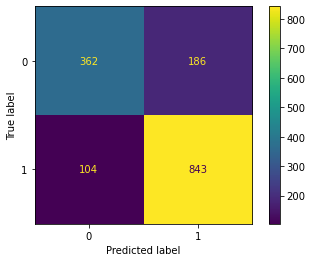
\includegraphics[width=\textwidth]{kaggle_figs/rf_cm.png}
         \subcaption{Random Forest Classifier}
         \label{fig:rf_cm}
     \end{minipage}
     \begin{minipage}{0.4\textwidth}
         \centering
         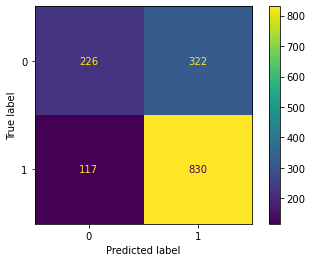
\includegraphics[width=\textwidth]{kaggle_figs/lr_cm.png}
         \subcaption{Logistic Regression Classifier}
         \label{fig:lr_cm}
     \end{minipage}
        \caption{Confusion Matrices of different classifiers}
        \label{fig:cm}
\end{figure}

\subsection{Fixing Mistakes}
\begin{itemize}
    \item Dropping features I couldn't engineer - There are features like \texttt{Property\_type} and \texttt{Review\_score\_rating} which I have dropped from the analysis. Given more time, I would like to work on them further and try to include them in the analysis.
    \item \texttt{Property\_type} had many property types and some of them seemed to be very similar to each other. I tried to study these property types in greater detail, combine the similar ones together and categorize them for the analysis. But together in train and test, there were just too many types and including them was leading to sparse data. So I decided to drop them for this analysis.
    \item \texttt{Review\_score\_rating} - This feature had missing values and I did not want to impute them with mean or 0 values. So I built a regression model which predicted the review scores based on other attributes. However, this did not particularly improve results while also taking up lot of computation resources. Intuitively, this meant that a house with similar facilites should have similar reviews, but this might not be true in practice. I decided to drop the feature for this analysis.
\end{itemize}
\section*{Citations}
\bibliography{references}
\section*{Code and Appendix}
\begin{lstlisting}
Put your code here.
\end{lstlisting}

\end{document}
